\documentclass{beamer}
\usetheme[sectionpage=none]{metropolis}

\usepackage{tikz}
\usepackage{tkz-graph}
\usetikzlibrary{calc,shapes.multipart,chains,arrows,backgrounds}

\usepackage{minted}
\setminted[haskell]{escapeinside=@@}
\newcommand{\hs}{\mintinline{haskell}}

\usepackage{mathtools}

\renewcommand{\epsilon}{\varepsilon}
\newcommand{\eps}{\epsilon}
\newcommand{\connect}{\rightarrow}


\title{Algebraic Graphs with Class}
\author{Christoph Madlener}
\date{01.06.2021}

\begin{document}
\begin{frame}[plain]
  \titlepage
\end{frame}

\section{Introduction}
\begin{frame}[fragile]
  \frametitle{Introduction}

  \begin{columns}
    \begin{column}{.6\linewidth}
      \onslide<1->
      \centering
      \begin{tikzpicture}
        \draw[draw=black,fill=mDarkTeal!30,rounded corners] (-1.25,-1.5) rectangle ++ (3,3);
        \tikzset{EdgeStyle/.style = {->, bend left}}
        \Vertices{circle}{3,1,2}
        \Edge(1)(2)
        \Edge(2)(1)
        \Edge(1)(3)
      \end{tikzpicture}
      $G_1$\onslide<3->${} = \Big(\big\{1,2,3\big\}, \big\{(1,2), (1,3), (2,1)\big\}\Big)$
    \end{column}
    \begin{column}{.35\linewidth}
      \onslide<2->
      \[
        G = (V,E) \text{ s.t. } \alert{E \subseteq V \times V}
      \]
    \end{column}
  \end{columns}

  \onslide<4->
  \begin{alertblock}{In Haskell?}
    \begin{minted}{haskell}
    data G a = G { vs :: Set a, es :: Set (a,a) }
    \end{minted}
    \onslide<5->
    \hs{g1 = G [1,2,3] [(1,2), (1,3), (2,1)]} 
    \onslide<6->
    \hs{g2 = G [1,2] [(1,3)]} \hspace{15mm}{\color{red} $E \nsubseteq V \times V$}
  \end{alertblock}
\end{frame}


\begin{frame}
  \frametitle{\texttt{containers} \& \texttt{fgl}}
  \begin{columns}[t]
    \begin{column}{.35\textwidth}
      \onslide<+->
      \begin{exampleblock}{\texttt{containers}}
        adjacency lists
        
        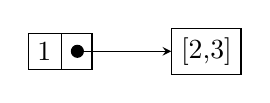
\begin{tikzpicture}[vertex/.style={rectangle split, rectangle split parts=2,
            draw, rectangle split horizontal}, >=stealth, start chain,
          list/.style={rectangle,draw}]

          \node[vertex,on chain] (1) {1};
          \node[list,on chain] (2) {[2,3]};
          \draw[*->] let \p1 = (1.two), \p2 = (1.center) in (\x1,\y2) -- (2);
        \end{tikzpicture}
        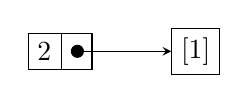
\begin{tikzpicture}[vertex/.style={rectangle split, rectangle split parts=2,
            draw, rectangle split horizontal}, >=stealth, start chain,
          list/.style={rectangle,draw}]

          \node[vertex,on chain] (1) {2};
          \node[list,on chain] (2) {[1]};
          \draw[*->] let \p1 = (1.two), \p2 = (1.center) in (\x1,\y2) -- (2);
        \end{tikzpicture}
        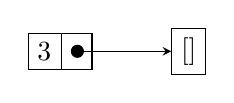
\begin{tikzpicture}[vertex/.style={rectangle split, rectangle split parts=2,
            draw, rectangle split horizontal}, >=stealth, start chain,
          list/.style={rectangle,draw}]

          \node[vertex,on chain] (1) {3};
          \node[list,on chain] (2) {[]};
          \draw[*->] let \p1 = (1.two), \p2 = (1.center) in (\x1,\y2) -- (2);
        \end{tikzpicture}
      \end{exampleblock}
    \end{column}
    \begin{column}{.55\textwidth}
      \onslide<+->
      \begin{exampleblock}{\texttt{fgl}}
        \textit{inductive graphs}
        \begin{itemize}
        \item inductive datatype: Context of a vertex + Graph
        \end{itemize}
      \end{exampleblock}
    \end{column}
  \end{columns}
  \onslide<+->
  
  \begin{alertblock}{$E \subseteq V \times V$ ?}
    \onslide<+->
    \begin{itemize}
    \item partial functions \textrightarrow runtime errors
    \end{itemize}
  \end{alertblock}
\end{frame}

\begin{frame}[fragile]
  \frametitle{Algebraic Graphs}
  \onslide<+->
  \begin{itemize}
  \item complete and \alert{consistent} graph representation
  \item simple construction primitives (\emph{``the core''})
  \end{itemize}
  \onslide<+->
  \begin{alertblock}{Achieved by the datatype}
    \begin{minted}{haskell}
    data Graph a = Empty
                 | Vertex a
                 | Overlay (Graph a) (Graph a)
                 | Connect (Graph a) (Graph a)
    \end{minted}
  \end{alertblock}
\end{frame}

\begin{frame}
  \frametitle{Empty ($\eps$) \& Vertex}
  \begin{columns}[t]
    \onslide<+->
    \begin{column}{.45\textwidth}
      \begin{exampleblock}{Empty - $\eps$}
        \vspace{5pt}
        \centering 
        \begin{tikzpicture}
          \draw[draw=black,fill=mDarkTeal!30, rounded corners] (0,0) rectangle ++ (3,3);
        \end{tikzpicture}
        
        \hs{Empty} ${} = \eps = (\emptyset, \emptyset)$
      \end{exampleblock}
    \end{column}
    \onslide<+->
    \begin{column}{.45\textwidth}
      \begin{exampleblock}{Vertex}
        \vspace{5pt}
        \centering
        \begin{tikzpicture}
          \draw[draw=black,fill=mDarkTeal!30, rounded corners] (0,0) rectangle ++ (3,3);
          \Vertex[x=1.5,y=1.5]{1};
        \end{tikzpicture}

        \hs{Vertex 1} ${} = (\{1\}, \emptyset)$
      \end{exampleblock}
    \end{column}
  \end{columns}
\end{frame}

\begin{frame}
  \frametitle{Overlay ($+$)}
  \begin{columns}
    \begin{column}{.25\textwidth}
      \centering
      \begin{tikzpicture}[scale=0.9]
        \draw[draw=black,fill=mDarkTeal!30, rounded corners] (0,0) rectangle ++ (3,3);
        \Vertex[x=0.75,y=2.25]{1};
        \Vertex[x=0.75,y=0.75]{2};
        \Vertex[x=2.25,y=1.5]{3};
        \Edge[style={bend right,->}](1)(2);
        \Loop[dir=SOEA, dist=0.8cm](3);
      \end{tikzpicture}
    \end{column}
    \begin{column}{.1\textwidth}
      \centering
      {\LARGE $+$}
    \end{column}
    \begin{column}{.25\textwidth}
      \centering
      \begin{tikzpicture}[scale=0.9]
        \draw[draw=black,fill=mDarkTeal!30, rounded corners] (0,0) rectangle ++ (3,3);
        \Vertex[x=0.75,y=0.75]{2};
        \Vertex[x=2.25,y=1.5]{3};
        \Edge[style={bend right,->}](2)(3);
        \Loop[dir=SOEA, dist=0.8cm](3);
      \end{tikzpicture}
    \end{column}
    \begin{column}{.1\textwidth}
      \centering
      {\LARGE $=$}
    \end{column}
    \begin{column}{.25\textwidth}
      \centering
      \begin{tikzpicture}[scale=0.9]
        \draw[draw=black,fill=mDarkTeal!30, rounded corners] (0,0) rectangle ++ (3,3);
        \Vertex[x=0.75,y=2.25]{1};
        \Vertex[x=0.75,y=0.75]{2};
        \Vertex[x=2.25,y=1.5]{3};
        \Edge[style={bend right,->}](1)(2);
        \Edge[style={bend right,->}](2)(3);
        \Loop[dir=SOEA, dist=0.8cm](3);
      \end{tikzpicture}
    \end{column}
  \end{columns}
  \[
    (V_1, E_1) + (V_2, E_2) \coloneqq (V_1 \cup V_2, E_1 \cup E_2)
  \]
\end{frame}

\begin{frame}
  \frametitle{Connect ($\connect$ / $*$)}
  \begin{columns}
    \begin{column}{.25\textwidth}
      \centering
      \begin{tikzpicture}[scale=0.9]
        \draw[draw=black,fill=mDarkTeal!30, rounded corners] (0,0) rectangle ++ (3,3);
        \Vertex[x=0.75,y=2.25]{1};
        \Vertex[x=0.75,y=0.75]{2};
        \Edge[style={bend right,->}](1)(2);
      \end{tikzpicture}
    \end{column}
    \begin{column}{.1\textwidth}
      \centering
      {\LARGE $\connect$}
    \end{column}
    \begin{column}{.25\textwidth}
      \centering
      \begin{tikzpicture}[scale=0.9]
        \draw[draw=black,fill=mDarkTeal!30, rounded corners] (0,0) rectangle ++ (3,3);
        \Vertex[x=0.75,y=2.25]{1};
        \Vertex[x=2.25,y=1.5]{3};
        \Edge[style={bend left,->}](1)(3);
      \end{tikzpicture}
    \end{column}
    \begin{column}{.1\textwidth}
      \centering
      {\LARGE $=$}
    \end{column}
    \begin{column}{.25\textwidth}
      \centering
      \begin{tikzpicture}[scale=0.9]
        \draw[draw=black,fill=mDarkTeal!30, rounded corners] (0,0) rectangle ++ (3,3);
        \Vertex[x=0.75,y=2.25]{1};
        \Vertex[x=0.75,y=0.75]{2};
        \Vertex[x=2.25,y=1.5]{3};

        \Loop[dist=0.8cm](1)
        \Edge[style={bend left,->}](1)(3);
        \tikzset{EdgeStyle/.style={bend right,->}}
        \Edge(1)(2);
        \Edge(2)(1);
        \Edge(2)(3);
      \end{tikzpicture}
    \end{column}
  \end{columns}
  \[
    (V_1, E_1) \connect (V_2, E_2) \coloneqq (V_1 \cup V_2, E_1 \cup E_2 \cup
    V_1 \times V_2)
  \] 
\end{frame}

\section{Graph Construction \& Transformation}
\begin{frame}[fragile]
  \frametitle{Graph Construction}
  \onslide<+->
  \begin{minted}{haskell}
vertices :: [a] -> Graph a
vertices = foldr Overlay Empty . map Vertex   
  \end{minted}
  \onslide<+->
  \vspace{5mm}
  \begin{columns}
    \begin{column}{.3\textwidth}
      \hs{vertices [1,2,3,4]}
    \end{column}
    \begin{column}{.05\textwidth}
      {\LARGE $=$}
    \end{column}
    \begin{column}{.4\textwidth}
      \begin{tikzpicture}
        \draw[draw=black,fill=mDarkTeal!30,rounded corners] (0,0) rectangle ++ (3,3);
        \Vertex[x=0.75,y=2.25]{1};
        \Vertex[x=0.75,y=0.75]{2};
        \Vertex[x=2.25,y=0.75]{3};
        \Vertex[x=2.25,y=2.25]{4};
      \end{tikzpicture}
    \end{column}
  \end{columns}
\end{frame}

\begin{frame}[fragile]
  \frametitle{Graph Construction}
  \onslide<+->
  \begin{minted}{haskell}
edge :: a -> a -> Graph a
edge u v = Connect (Vertex u) (Vertex v)
  \end{minted}
  \onslide<+->
  \begin{minted}{haskell}
edges :: [(a,a)] -> Graph a
edges = foldr Overlay Empty . map (uncurry edge)
  \end{minted}
  \onslide<+->
  \vspace{5mm}
  \begin{columns}
    \begin{column}{.3\textwidth}
      \hs{edges [(1,2),(3,4)]}
    \end{column}
    \begin{column}{.05\textwidth}
      {\LARGE $=$}
    \end{column}
    \begin{column}{.4\textwidth}
      \begin{tikzpicture}
        \draw[draw=black,fill=mDarkTeal!30,rounded corners] (0,0) rectangle ++ (3,3);
        \Vertex[x=0.75,y=2.25]{1};
        \Vertex[x=0.75,y=0.75]{2};
        \Vertex[x=2.25,y=0.75]{3};
        \Vertex[x=2.25,y=2.25]{4};
        \tikzset{EdgeStyle/.style={->}}
        \Edge(1)(2);
        \Edge(3)(4);
      \end{tikzpicture}
    \end{column}
  \end{columns}
\end{frame}

\begin{frame}[fragile]
  \frametitle{Graph Construction}
  \onslide<+->
  \begin{minted}{haskell}
graph :: [a] -> [(a,a)] -> Graph a
graph vs es = Overlay (vertices vs) (edges es)
  \end{minted}
  \onslide<+->
  \vspace{5mm}
  \begin{columns}
    \begin{column}{.3\textwidth}
      \hs{graph [1] [(3,4)]}
    \end{column}
    \begin{column}{.05\textwidth}
      {\LARGE $=$}
    \end{column}
    \begin{column}{.4\textwidth}
      \begin{tikzpicture}
        \draw[draw=black,fill=mDarkTeal!30,rounded corners] (0,0) rectangle ++ (3,3);
        \Vertex[x=0.75,y=2.25]{1};
        \Vertex[x=2.25,y=0.75]{3};
        \Vertex[x=2.25,y=2.25]{4};
        \tikzset{EdgeStyle/.style={->}}
        \Edge(3)(4);
      \end{tikzpicture}
    \end{column}
  \end{columns}
\end{frame}

\begin{frame}[fragile]
  \frametitle{Graph Transformation - Functor}
  \begin{exampleblock}{Functor}
    \onslide<+->
    \begin{minted}{haskell}
instance Functor Graph where
  ...
  fmap f (Vertex u) = Vertex (f u)
  ...
    \end{minted}
    \onslide<+->
    \vspace{5mm}
    \begin{columns}
      \begin{column}{.15\textwidth}
        \hs{fmap (+1)}
      \end{column}
      \begin{column}{.25\textwidth}
        \begin{tikzpicture}[scale=0.9]
          \draw[draw=black,fill=mDarkTeal!30,rounded corners] (0,0) rectangle ++ (3,3);
          \Vertex[x=0.75,y=2.25]{1};
          \Vertex[x=0.75,y=0.75]{2};
          \Vertex[x=2.25,y=1.5]{3};
          \Edge[style={bend right,->}](1)(2);
          \Edge[style={bend right,->}](2)(3);
          \Loop[dir=SOEA, dist=0.8cm](3);
        \end{tikzpicture}
      \end{column}
      \begin{column}{.05\textwidth}
        {\LARGE $=$}
      \end{column}
      \begin{column}{.25\textwidth}
        \begin{tikzpicture}[scale=0.9]
          \draw[draw=black,fill=mDarkTeal!30,rounded corners] (0,0) rectangle ++ (3,3);
          \Vertex[x=0.75,y=2.25]{2};
          \Vertex[x=0.75,y=0.75]{3};
          \Vertex[x=2.25,y=1.5]{4};

          \Edge[style={bend right,->}](2)(3);
          \Edge[style={bend right,->}](3)(4);
          \Loop[dir=SOEA, dist=0.8cm](4);
        \end{tikzpicture}
      \end{column}
    \end{columns}
  \end{exampleblock}
\end{frame}

\begin{frame}[fragile]
  \frametitle{Graph Transformation - Merging Vertices}
  \onslide<+->
  \begin{minted}{haskell}
mergeVs :: (a -> Bool) -> a -> Graph a -> Graph a
mergeVs p v = fmap $ \u -> if p u then v else u
  \end{minted}
  % $
  \onslide<+->
  \vspace{5mm}
  \begin{columns}
    \begin{column}{.25\textwidth}
      \hs{mergeVs (>1) 4}
    \end{column}
    \begin{column}{.25\textwidth}
      \begin{tikzpicture}[scale=0.9]
        \draw[draw=black,fill=mDarkTeal!30,rounded corners] (0,0) rectangle ++ (3,3);
        \Vertex[x=0.75,y=2.25]{1};
        \Vertex[x=0.75,y=0.75]{2};
        \Vertex[x=2.25,y=1.5]{3};

        \Edge[style={bend right,->}](1)(2);
        \Edge[style={bend right,->}](2)(3);
      \end{tikzpicture}
    \end{column}
    \begin{column}{.05\textwidth}
      {\LARGE $=$}
    \end{column}
    \begin{column}{.25\textwidth}
      \begin{tikzpicture}[scale=0.9]
        \draw[draw=black,fill=mDarkTeal!30,rounded corners] (0,0) rectangle ++ (3,3);
        \Vertex[x=0.75,y=2.25]{1};
        \Vertex[x=1.5,y=1.125]{4};
        \Edge[style={bend right,->}](1)(4);
        \Loop[dir=SOEA, dist=0.8cm](4);
      \end{tikzpicture}
    \end{column}
  \end{columns}
\end{frame}

\begin{frame}[fragile]
  \frametitle{Graph Transformation - Monad}
  \onslide<+->
  \begin{minted}{haskell}
instance Monad Graph where
  ...
  (Vertex u) >>= f = f u
  ...
  \end{minted}
  \onslide<+->
  \begin{minted}{haskell}
splitVertex :: (a -> Bool) -> [a] -> Graph a
splitVertex p vs = g >>= \u -> if p u
                               then vertices vs
                               else Vertex u
  \end{minted}
  \onslide<+->
  \vspace{5mm}
  \begin{columns}
    \begin{column}{.35\textwidth}
      \hs{splitVertex 4 [2,3]}
    \end{column}
    \begin{column}{.25\textwidth}
      \begin{tikzpicture}[scale=0.9]
        \draw[draw=black,fill=mDarkTeal!30,rounded corners] (0,0) rectangle ++ (3,3);
        \Vertex[x=0.75,y=2.25]{1};
        \Vertex[x=1.5,y=1.125]{4};

        \Edge[style={bend right,->}](1)(4);
        \Loop[dir=SOEA, dist=0.8cm](4);
      \end{tikzpicture}
    \end{column}
    \begin{column}{.02\textwidth}
      {\LARGE $=$}
    \end{column}
    \begin{column}{.25\textwidth}
      \begin{tikzpicture}[scale=0.9]
        \draw[draw=black,fill=mDarkTeal!30,rounded corners] (0,0) rectangle ++ (3,3);
        \Vertex[x=0.75,y=2.25]{1};
        \Vertex[x=0.75,y=0.75]{2};
        \Vertex[x=2.25,y=1.5]{3};
        \Edge[style={bend right,->}](1)(2);
        \Edge[style={bend left,->}](1)(3);
        \Edge[style={bend left,->}](2)(3);
        \Edge[style={bend left,->}](3)(2);
        \Loop[dir=SOWE,dist=0.8cm](2);
        \Loop[dir=SOEA,dist=0.8cm](3);
      \end{tikzpicture}
    \end{column}
  \end{columns}
\end{frame}


\begin{frame}[fragile]
  \frametitle{Graph Transformation - MonadPlus}
  \onslide<+->
  \begin{minted}{haskell}
instance Graph MonadPlus where
  mzero = Empty
  mplus = Overlay
  \end{minted}
  \onslide<+->
  \begin{minted}{haskell}
induce :: (a -> Bool) -> Graph a -> Graph a
induce = mfilter    
  \end{minted}
  \onslide<+->
  \vspace{5mm}
  \begin{columns}
    \begin{column}{.2\textwidth}
      \hs{induce even}
    \end{column}
    \begin{column}{.25\textwidth}
      \begin{tikzpicture}[scale=0.9]
        \draw[draw=black,fill=mDarkTeal!30,rounded corners] (0,0) rectangle ++ (3,3);
        \Vertex[x=0.75,y=2.25]{1};
        \Vertex[x=0.75,y=0.75]{2};
        \Vertex[x=2.25,y=0.75]{3};
        \Vertex[x=2.25,y=2.25]{4};
        \Edge[style={bend right,->}](1)(2);
        \Edge[style={bend left,->}](2)(4);
        \Edge[style={bend left,->}](4)(3);
      \end{tikzpicture}
    \end{column}
    \begin{column}{.05\textwidth}
      {\LARGE $=$}
    \end{column}
    \begin{column}{.25\textwidth}
      \begin{tikzpicture}[scale=0.9]
        \draw[draw=black,fill=mDarkTeal!30,rounded corners] (0,0) rectangle ++ (3,3);
        \Vertex[x=0.75,y=0.75]{2};
        \Vertex[x=2.25,y=2.25]{4};
        \Edge[style={bend left,->}](2)(4);
      \end{tikzpicture}
    \end{column}
  \end{columns}
\end{frame}

\section{Algebra}
\begin{frame}
  \frametitle{\textsc{Algebraic} Graphs}
  \onslide<+->
  \begin{alertblock}{Overlay ($+$) and connect ($\connect$) almost form a semiring over graphs}
    \begin{itemize}[<+->]
    \item $(\mathcal{G}, +, \alert<5>{\eps})$ is an idempotent, commutative monoid
    \item $(\mathcal{G}, \connect, \alert<5>{\eps})$ is a monoid
    \item $\connect$ distributes over $+$ 
    \end{itemize}
  \end{alertblock}

  \begin{itemize}[<+->]
  \item ``shared'' identity \alert{$\eps$}
  \item no ``zero'' for $\connect$ (i.e.\ $g \connect 0 = 0$)
  \end{itemize}
\end{frame}

\begin{frame}
  \frametitle{Decomposition}
  \onslide<+->
  Additional axiom for algebra of graphs
  \[
    x \connect y \connect z = x \connect y + x \connect z + y \connect z
  \]
  \onslide<+->
  \begin{columns}
    \begin{column}{.25\textwidth}
      \begin{tikzpicture}[scale=0.7]
        \draw[draw=black,fill=mDarkTeal!30,rounded corners] (0.45,0.45) rectangle ++ (1.1,1.1);
        \draw[draw=black,fill=mDarkTeal!30,rounded corners] (1.95,0.45) rectangle ++ (1.1,1.1);
        \draw[draw=black,fill=mDarkTeal!30,rounded corners] (3.45,0.45) rectangle ++ (1.1,1.1);
        \draw[draw=black,rounded corners] (0.4,0.4) rectangle ++ (2.7,1.2);
        \draw[draw=black,rounded corners] (0.35, 0.35) rectangle ++ (4.3,1.3);
        \draw[->] (1.55,1) -- (1.95,1);
        \draw[->] (3.1,1) -- (3.45,1);
        \Vertex[x=1,y=1]{1};
        \Vertex[x=2.5,y=1]{2};
        \Vertex[x=4,y=1]{3};
      \end{tikzpicture}
    \end{column}
    \onslide<+->
    \begin{column}{.02\textwidth}
      {\LARGE $=$}
    \end{column}
    \begin{column}{.17\textwidth}
      \begin{tikzpicture}[scale=0.7]
        \draw[draw=black,fill=mDarkTeal!30,rounded corners] (0,0) rectangle ++ (3,3);
        \Vertex[x=0.75,y=2.25]{1};
        \Vertex[x=0.75,y=0.75]{2};
        \Vertex[x=2.25,y=1.5]{3};
        \tikzset{EdgeStyle/.style={->}}
        \Edge(1)(2);
        \Edge(1)(3);
        \Edge(2)(3);
      \end{tikzpicture}
    \end{column}
    \onslide<+->
    \begin{column}{.02\textwidth}
      {\LARGE $=$}
    \end{column}
    \begin{column}{.05\textwidth}
      \begin{tikzpicture}[scale=0.7]
        \draw[draw=black,fill=mDarkTeal!30,rounded corners] (0.2,1.7) rectangle ++ (1.1,1.1);
        \draw[draw=black,fill=mDarkTeal!30,rounded corners] (0.2,0.2) rectangle ++ (1.1,1.1);
        \draw[draw=black,rounded corners] (0.15,0.15) rectangle ++ (1.2,2.7);
        \draw[->] (0.75,1.7) -- (0.75,1.3);
        \Vertex[x=0.75,y=2.25]{1};
        \Vertex[x=0.75,y=0.75]{2};
      \end{tikzpicture}
    \end{column}
    \begin{column}{.02\textwidth}
      {\LARGE $+$}
    \end{column}
    \begin{column}{.2\textwidth}
      \begin{tikzpicture}[scale=0.7]
        \draw[draw=black,fill=mDarkTeal!30,rounded corners] (0.45,0.45) rectangle ++ (1.1,1.1);
        \draw[draw=black,fill=mDarkTeal!30,rounded corners] (1.95,0.45) rectangle ++ (1.1,1.1);
        \draw[draw=black,rounded corners] (0.4,0.4) rectangle ++ (2.7,1.2);
        \draw[->] (1.55,1) -- (1.95,1);
        \Vertex[x=1,y=1]{1};
        \Vertex[x=2.5,y=1]{3};
      \end{tikzpicture}
      
      \vspace{5mm}
      \begin{tikzpicture}[scale=0.7]
        \draw[draw=black,fill=mDarkTeal!30,rounded corners] (0.45,0.45) rectangle ++ (1.1,1.1);
        \draw[draw=black,fill=mDarkTeal!30,rounded corners] (1.95,0.45) rectangle ++ (1.1,1.1);
        \draw[draw=black,rounded corners] (0.4,0.4) rectangle ++ (2.7,1.2);
        \draw[->] (1.55,1) -- (1.95,1);
        \Vertex[x=1,y=1]{1};
        \Vertex[x=2.5,y=1]{3};
      \end{tikzpicture}
    \end{column}
  \end{columns}
\end{frame}

\begin{frame}
  \frametitle{Subgraph Relation}
  Define subgraphs in terms of $(+)$ and equality:
  \[
    x \sqsubseteq y \iff x + y = y
  \]
\end{frame}

\begin{frame}
  \frametitle{Beyond Directed Graphs}
  \onslide<+->
  \begin{alertblock}{Obtain other classes of graphs by modifying the set of
      axioms:}
    \begin{itemize}[<+->]
    \item Undirected graphs: $\leftrightarrow$ is commutative ($x
      \leftrightarrow y = y \leftrightarrow x$)
    \item Reflexive graphs: $x = x \connect x$
    \item Transitive graphs:
      \[
        y \neq \eps \Rightarrow (x \connect y) + (y \connect z) + (x \connect z) = (x
        \connect y) + (y \connect z)
      \]
    \item Preorders (reflexive + transitive), equivalence relations (preorder +
      undirected)
    \item Hypergraphs
    \end{itemize}
  \end{alertblock}
\end{frame}

\begin{frame}
  \frametitle{Graph Equality}
  \onslide<+->
  Structural equality is not suitable: \hs{Overlay (Vertex 1) Empty == Vertex 1}
  \onslide<+->
  \begin{alertblock}{\hs{Eq} instance for Algebraic Graphs}
    \begin{itemize}
    \item Current implementation: build adjacency map
    \item<+-> Possible approach: \emph{minimize} graph expressions
      \textrightarrow \emph{Modular Graph Decomposition}
    \end{itemize}
  \end{alertblock}
\end{frame}

\begin{frame}[fragile]
  \frametitle{Compact Representation for Dense Graphs}
  \onslide<+->
  Fully connected (undirected) graph
  \begin{minted}{haskell}
clique :: [a] -> Graph a
clique = foldr Connect Empty . map Vertex
  \end{minted}
  \onslide<+->
  \begin{itemize}
  \item \alert{Linear size representation}
  \item quadratic in size when using e.g.\ adjacency map
  \end{itemize}
  \onslide<+->
  \begin{exampleblock}{Open question}
    \begin{itemize}
    \item Can we exploit this compact representation, i.e.\ find algorithms that
      work directly on algebraic graphs?
    \end{itemize}
  \end{exampleblock}
\end{frame}

\begin{frame}
  \frametitle{Formal Verification}
  \begin{itemize}[<+->]
  \item using Isabelle/HOL
  \item inductive datatype \textrightarrow{} proofs by induction, \texttt{auto}
  \item \texttt{quotient\_type} (think \hs{Eq} instance) based on tuple representation
  \end{itemize}
  \onslide<+->
  \begin{exampleblock}{Future work}
    \begin{itemize}
    \item Minimization
    \item Algorithms, applications beyond graph construction/transformation
    \end{itemize}
  \end{exampleblock}
\end{frame}

\section{Class/Locale}
\begin{frame}[fragile]
  \frametitle{Algebraic Graphs with \textsc{Class}}
  \onslide<+->
  \begin{minted}{haskell}
class Graph g where
  type Vertex g
  empty :: g
  vertex :: Vertex g -> g
  overlay :: g -> g -> g
  connect :: g -> g -> g
  \end{minted}
  \onslide<+->
  \alert{\textrightarrow Polymorphic graph construction/transformation library}
\end{frame}

\begin{frame}
  \frametitle{Formal Verification}
  \begin{itemize}[<+->]
  \item define \texttt{locale} in Isabelle/HOL (think Haskell class + axioms)
  \item equational reasoning for simple statements
    \[
      \hs{vertices xs} \sqsubseteq \hs{clique xs}
    \]
  \item formal proof of completeness and consistency
  \end{itemize}
\end{frame}

\begin{frame}
  \frametitle{Formal Verification}
  \begin{itemize}[<+->]
  \item formalized material on vertex walks, reachability
  \item probably additional axioms required ($\eps \neq \hs{vertex u}$)
  \end{itemize}
  \onslide<+->
  \begin{exampleblock}{Future work}
    \begin{itemize}
    \item more graph theory (e.g.\ strongly connected components)
    \item algorithms
    \end{itemize}
    \onslide<+->
    \textrightarrow{} \alert{\emph{Verified}} polymorphic graph library
  \end{exampleblock}
\end{frame}

\section{Conclusion}
\begin{frame}
  \frametitle{Conclusion}
  \begin{alertblock}{}
  \begin{itemize}
  \item<+-> alternative approach to graph construction/transformation
    \begin{itemize}
    \item small core of primitives - safe and complete
    \end{itemize}
  \item<+-> two main directions for future work
    \begin{enumerate}
    \item exploit compact representation/other applications of data type
    \item exploit polymorphism of type class/locale
    \end{enumerate}
  \end{itemize}
  \end{alertblock}
\end{frame}
\end{document}